\chapter{有限元逼近}\label{ch:3}
\SourcePage{86}

本章介绍经典有限元逼近的性质,着重说明这一方法的三个基本方面：区域 \(\Omega\) 可以剖分,可以构造由分片多项式组成的有限维子空间,而且这个子空间具有由小支集函数组成的基.随后引入插值算子,并估计插值误差.最后讨论有限元子空间上的几个投影算子及其逼近性质.

这些结果为推导有限元逼近的误差估计奠定基础.后续各章将对偏微分方程作有限元逼近,并用到这些估计.

\section{剖分}\label{sec:3.1}

设 \(\Omega\subset\mathbb R^d\),\(d=2,3\),是一个多边形域或多面体域,即 \(\Omega\) 是有界连通开集,且其闭包 \(\overline\Omega\) 是有限个多边形或多面体的并.这里考虑有限分解
\begin{equation}\label{eq:3.1.1}
  \overline\Omega=\bigcup_{K\in\mathcal T_h}K,
\end{equation}
其中
\begin{align}
  &\text{每个 \(K\) 都是多面体(二维时为多边形),且 \(\mathring K\ne\varnothing\)；}
  \label{eq:3.1.2}\\
  &\mathring K_1\cap\mathring K_2=\varnothing
    \qquad\text{对任意不同的 \(K_1,K_2\in\mathcal T_h\)；}
  \label{eq:3.1.3}\\
  &\begin{aligned}
    &\text{若 \(F=K_1\cap K_2\ne\varnothing\),其中 \(K_1,K_2\) 是 \(\mathcal T_h\) 的不同单元,}\\
    &\text{则 \(F\) 是 \(K_1\) 与 \(K_2\) 的一个公共面、公共边或公共顶点；}
  \end{aligned}
  \label{eq:3.1.4}\\
  &\operatorname{diam}(K)\le h\qquad\text{对每个 \(K\in\mathcal T_h\).}
  \label{eq:3.1.5}
\end{align}
称 \(\mathcal T_h\) 为 \(\overline\Omega\) 的一个\emph{剖分}(\figref{fig:3.1.1}给出了符合条件和不符合条件的构形).

为简化讨论,下面还假设 \(\mathcal T_h\) 中每个单元 \(K\) 都可写成 \(K=T_K(\widehat K)\),其中 \(\widehat K\) 是参考多面体,\SourcePage{87}\(T_K\) 是适当的可逆仿射映射,即 \(T_K(\widehat{\boldsymbol{x}})=B_K\widehat{\boldsymbol{x}}+\boldsymbol{b}_K\),\(B_K\) 为非奇异矩阵.

\begin{figure}[htbp]
  \centering
  \includegraphics[page=87,pagebox=cropbox,trim=81.17bp 511.00bp 72.17bp 84.33bp,clip,width=.651\paperwidth]{../input/source/Numerical Approximation of Partial Differential Equations.pdf}
  \caption{符合条件的剖分(左)和不符合条件的剖分(右)}\label{fig:3.1.1}
\end{figure}

我们只考虑以下两种情形：
\begin{equation}\label{eq:3.1.6}
  \begin{aligned}
    &\text{\(\widehat K\) 为单位 \(d\)-单纯形,即 \(d=2\) 时顶点为 \((0,0),(1,0),(0,1)\) 的三角形,}\\
    &\text{或 \(d=3\) 时顶点为 \((0,0,0),(1,0,0),(0,1,0),(0,0,1)\) 的四面体.}\\
    &\text{因此每个 \(K=T_K(\widehat K)\) 都是三角形或四面体.}
  \end{aligned}
\end{equation}
\begin{equation}\label{eq:3.1.7}
  \begin{aligned}
    &\text{\(\widehat K\) 为单位 \(d\)-立方体 \([0,1]^d\).因此每个 \(K=T_K(\widehat K)\) 都是平行四边形}\\
    &\text{(\(d=2\) 时)或平行六面体(\(d=3\) 时).}
  \end{aligned}
\end{equation}
在后一种情形中,如果对每个 \(K\in\mathcal T_h\),定义仿射变换 \(T_K\) 的矩阵 \(B_K\) 都是对角矩阵,那么剖分就由 \(d\) 维矩形组成.

要处理一般四边形或六面体,变换 \(T_K\) 仍需可逆,但其各分量要允许采用关于每个变量 \(x_1,\ldots,x_d\) 分别为一次的多项式,也就不再局限于仿射映射.本书不考虑这种情形.有兴趣的读者可参见\BookCite{ciarlet1978}{Ciarlet(1978}、\BookCite{ciarlet1991}{1991)},其中给出了有限元的一般逼近理论.

\section{分片多项式子空间}\label{sec:3.2}

有限元法的第二个基本方面,是根据所考虑的具体问题确定一个有限维空间 \(X_h\),使之能够适当地逼近无穷维空间 \(X\).

这里的关键是 \(v_h\in X_h\) 为分片多项式函数.也就是说,对每个 \(K\in\mathcal T_h\),空间
\[
  P_K:=\{v_h|_K\mid v_h\in X_h\}
\]
由代数多项式组成.

更确切地说,记 \(\mathbb P_k\)(\(k\ge0\))为变量 \(x_1,\ldots,x_d\) 的总次数不超过 \(k\) 的多项式空间,记 \(\mathbb Q_k\) 为关于每个变量 \(x_1,\ldots,x_d\) 的次数分别不超过 \(k\) 的多项式空间.容易算出
\SourcePage{88}
\begin{equation}\label{eq:3.2.1}
  \dim\mathbb P_k=\binom{d+k}{k},\qquad
  \dim\mathbb Q_k=(k+1)^d.
\end{equation}
此外,具有下列包含关系：
\[
  \mathbb P_k\subset\mathbb Q_k\subset\mathbb P_{dk}.
\]
还引入如下向量多项式空间：
\begin{equation}\label{eq:3.2.2}
  \mathbb D_k:=(\mathbb P_{k-1})^d+\boldsymbol{x}\mathbb P_{k-1},
    \qquad k\ge1,
\end{equation}
其中 \(\boldsymbol{x}\in\mathbb R^d\) 为自变量.若只在第二项中保留 \(k-1\) 次齐次多项式,所得空间相同,且这时两项构成直和.可以验证
\begin{equation}\label{eq:3.2.3}
  \dim\mathbb D_k=(d+k)\frac{(d+k-2)!}{(d-1)!(k-1)!},
\end{equation}
并且 \((\mathbb P_{k-1})^d\subset\mathbb D_k\subset(\mathbb P_k)^d\)(例如,见\BookCite{roberts-thomas1991}{Roberts 和 Thomas(1991)}).

\subsection{标量情形}\label{sec:3.2.1}

现在可以定义最常用的 \(X_h\) 空间了.

\begin{definition*}[三角形有限元空间]
在\eqref{eq:3.1.6}的情形下,令
\begin{equation}\label{eq:3.2.4}
  X_h=X_h^k:=\bigl\{v_h\in C^0(\overline\Omega)\mid
  v_h|_K\in\mathbb P_k\quad\forall K\in\mathcal T_h\bigr\},
  \qquad k\ge1,
\end{equation}
称为三角形有限元空间(三维时单元为四面体).
\end{definition*}

\begin{definition*}[平行六面体有限元空间]
在\eqref{eq:3.1.7}的情形下,令
\begin{equation}\label{eq:3.2.5}
  X_h=X_h^k:=\bigl\{v_h\in C^0(\overline\Omega)\mid
   (v_h|_K)\circ T_K\in\mathbb Q_k\quad\forall K\in\mathcal T_h\bigr\},
  \qquad k\ge1,
\end{equation}
称为平行六面体有限元空间(二维时单元为平行四边形).
\end{definition*}

注意,在\eqref{eq:3.2.5}的情形下,有限维空间 \(P_K=\{v_h|_K\mid v_h\in X_h^k\}\) 一般不同于 \(\mathbb Q_k\).例外是 \(K\) 为各边平行于坐标轴的矩形.此时可将 \(T_K\) 写成对角矩阵作用后再作平移,而 \(\mathbb Q_k\) 在这种变换下不变.一般有 \(\mathbb P_k\subset P_K\subset\mathbb P_{dk}\).

值得注意的是,无论是\eqref{eq:3.2.4}还是\eqref{eq:3.2.5}的情形,都有
\[
  X_h^k\subset H^1(\Omega)\qquad \forall k\ge1.
\]
事实上,这可由下列结果推出.为简便起见,此处及下文用 \(H^s(K)\) 代替 \(H^s(\mathring K)\).

\begin{proposition}[]{3.2.1}
函数 \(v\colon\Omega\to\mathbb R\) 属于 \(H^1(\Omega)\),当且仅当
\begin{enumerate}[label=\alph*.,leftmargin=*]
  \item 对每个 \(K\in\mathcal T_h\),有 \(v|_K\in H^1(K)\)；
  \item 对每个公共界面 \(F=K_1\cap K_2\),\(K_1,K_2\in\mathcal T_h\),\(v|_{K_1}\) 和 \(v|_{K_2}\) 在 \(F\) 上的迹相同.
\end{enumerate}
\end{proposition}

\begin{proof}
根据 a 项,定义函数 \(w_j\in L^2(\Omega)\)(\(j=1,\ldots,d\))如下：
\SourcePage{89}
\[
  w_j|_K:=D_j(v|_K)\qquad\forall K\in\mathcal T_h.
\]
要证明 \(v\in H^1(\Omega)\),只需证明 \(w_j=D_jv\).

利用 Green 公式(见\eqref{eq:1.3.3}),可对每个 \(\varphi\in\mathcal D(\Omega)\) 写出
\[
  \int_\Omega w_j\varphi
   =\sum_K\int_K w_j\varphi
   =-\sum_K\int_K(v|_K)D_j\varphi
    +\sum_K\int_{\partial K}(v|_K)\varphi n_{K,j},
\]
其中 \(\boldsymbol{n}_K\) 是 \(\partial K\) 上的单位外法向量.由于 \(\varphi\) 在 \(\partial\Omega\) 上为零,且在公共界面 \(F=K_1\cap K_2\) 上有 \(\boldsymbol{n}_{K_1}=-\boldsymbol{n}_{K_2}=:\boldsymbol{n}\),由 b 项可得
\[
  \int_\Omega w_j\varphi=-\int_\Omega vD_j\varphi
     +\sum_F\int_F(v|_{K_1}-v|_{K_2})\varphi n_j
     =-\int_\Omega vD_j\varphi,
\]
即 \(w_j=D_jv\).

反过来,若假定 \(v\in H^1(\Omega)\),a 项立即成立.此外,\(w_j=D_jv\).按前面同样的方式可得
\[
  \sum_F\int_F(v|_{K_1}-v|_{K_2})\varphi n_j=0
    \qquad \forall\varphi\in\mathcal D(\Omega),\quad j=1,\ldots,d,
\]
故 b 项成立.\hfill\(\square\)
\end{proof}

\subsection{向量情形}\label{sec:3.2.2}

\begin{definition*}[向量有限元空间]
在向量情形下,当 \(\widehat K\) 满足\eqref{eq:3.1.6}时,定义
\begin{equation}\label{eq:3.2.6}
  W_h^k:=\bigl\{\boldsymbol{v}_h\in H(\operatorname{div};\Omega)\mid
   \boldsymbol{v}_h|_K\in\mathbb D_k\quad\forall K\in\mathcal T_h\bigr\},
   \qquad k\ge1.
\end{equation}
\end{definition*}

对于\eqref{eq:3.1.7}的情形,也可以给出类似定义.有兴趣的读者可参见\BookCite{thomas1977}{Thomas(1977)}、\BookCite{raviart-thomas1977}{Raviart 和 Thomas(1977)}及\BookCite{nedelec1980}{Nédélec(1980)},本节不讨论这一情形.下列结果明确指出,要保证 \(\boldsymbol{v}_h\in W_h^k\),在单元 \(K\) 的边界上必须满足什么条件.

\begin{proposition}[]{3.2.2}
设 \(\boldsymbol{v}\colon\Omega\to\mathbb R^d\) 满足：
\begin{enumerate}[label=\alph*.,leftmargin=*]
  \item 对每个 \(K\in\mathcal T_h\),有 \(\boldsymbol{v}|_K\in(H^1(K))^d\)；
  \item 对每个公共界面 \(F=K_1\cap K_2\),\(K_1,K_2\in\mathcal T_h\),法向分量 \(\boldsymbol{n}\cdot\boldsymbol{v}|_{K_1}\) 和 \(\boldsymbol{n}\cdot\boldsymbol{v}|_{K_2}\) 在 \(F\) 上的迹相同.
\end{enumerate}
则 \(\boldsymbol{v}\in H(\operatorname{div};\Omega)\).反过来,若 \(\boldsymbol{v}\in H(\operatorname{div};\Omega)\) 且满足 a 项,则 b 项也成立.
\end{proposition}

\begin{proof}
定义 \(w\in L^2(\Omega)\) 如下：
\[
  w|_K:=\operatorname{div}(\boldsymbol{v}|_K)\qquad\forall K\in\mathcal T_h.
\]
利用 Green 公式(见\eqref{eq:1.3.4}),对每个 \(\varphi\in\mathcal D(\Omega)\),有
\SourcePage{90}
\[
  \begin{aligned}
    \langle\operatorname{div}\boldsymbol{v},\varphi\rangle
    &=-\int_\Omega\boldsymbol{v}\cdot\nabla\varphi
      =-\sum_K\int_K(\boldsymbol{v}|_K)\cdot\nabla\varphi\\
    &=\sum_K\int_K\operatorname{div}(\boldsymbol{v}|_K)\varphi
      -\sum_F\int_F(\boldsymbol{n}\cdot\boldsymbol{v}|_{K_1}-\boldsymbol{n}\cdot\boldsymbol{v}|_{K_2})\varphi
      =\int_\Omega w\varphi,
  \end{aligned}
\]
即 \(\operatorname{div}\boldsymbol{v}=w\).

另一方面,若 \(\boldsymbol{v}\in H(\operatorname{div};\Omega)\),则 \(w=\operatorname{div}\boldsymbol{v}\).由于 \(\boldsymbol{v}|_K\in(H^1(K))^d\),其在 \(F\) 上的迹有定义,并且
\[
  \sum_F\int_F(\boldsymbol{n}\cdot\boldsymbol{v}|_{K_1}-\boldsymbol{n}\cdot\boldsymbol{v}|_{K_2})\varphi=0
  \qquad \forall\varphi\in\mathcal D(\Omega),
\]
故 b 项成立.\hfill\(\square\)
\end{proof}

\section{自由度与形函数}\label{sec:3.3}

现在要为空间 \(X_h\) 构造一组基,并使基函数易于描述.

一个重要问题是为每个单元 \(K\) 选定一组\emph{自由度},即能唯一确定 \(\mathbb P_k\)、\(\mathbb Q_k\) 或 \(\mathbb D_k\) 中一个函数的参数.自由度的数目由\eqref{eq:3.2.1}或\eqref{eq:3.2.3}给出.

\subsection{标量情形：三角形有限元}\label{sec:3.3.1}

先考虑\eqref{eq:3.2.4}中 \(d=2\) 的情形.当 \(k=1\) 时,要确定 \(v_h|_K\),必须在每个单元 \(K\) 上选取三个自由度,并且还要满足 \(v_h\in C^0(\overline\Omega)\) 这一附加条件.最简单的选择是取 \(v_h\) 在各个 \(K\) 的顶点处的值.

注意,若考虑
\[
  Y_h^1:=\{v_h\in L^2(\Omega)\mid v_h|_K\in\mathbb P_1\quad\forall K\in\mathcal T_h\},
\]
而采用的不是\eqref{eq:3.2.4}定义的 \(X_h^1\),那么可以自由选取 \(K\) 上三个不共线的点,以函数在这些点的值作为自由度.这些点可以与顶点不同.例如,可以取三个内点作为节点,也可以取各边的中点.取各边中点显然只保证函数在中点处连续；若取内点,属于 \(Y_h^1\) 的函数在相邻三角形的公共边上一般会有两个不同的值.不过,下面回到\eqref{eq:3.2.4}的情形.

当 \(k=2\) 时,取函数在各顶点及各边中点的值作为单元的自由度.为说明更一般情形下的证明思路,下面证明这一点.记\SourcePage{91}三角形 \(K\) 的顶点为 \(\boldsymbol{a}^i\)(\(i=1,2,3\)),边的中点为 \(\boldsymbol{a}^{ij}\)(\(1\le i<j\le3\)).

\begin{proposition}[]{3.3.1}
一个函数 \(p\in\mathbb P_2\) 可由六个值唯一确定,即 \(p(\boldsymbol{a}^i)\)(\(1\le i\le3\))和 \(p(\boldsymbol{a}^{ij})\)(\(1\le i<j\le3\)).
\end{proposition}

\begin{proof}
由于自由度的数目等于 \(\mathbb P_2\) 的维数,即 \(6\),只需证明：若 \(p(\boldsymbol{a}^i)=p(\boldsymbol{a}^{ij})=0\) 对所有这些节点成立,则 \(p\equiv0\).

为此,注意 \(p\) 在每条边上的限制是一个一元二次多项式,它在三个不同的点处为零,所以在整条边上为零.于是可写成
\[
  p(\boldsymbol{x})=c\,p_1(\boldsymbol{x})p_2(\boldsymbol{x})p_3(\boldsymbol{x}),
\]
其中 \(p_i(\boldsymbol{x})\) 是一次多项式,每个在 \(K\) 的一条边上为零.由于 \(p\in\mathbb P_2\),故 \(c=0\).\hfill\(\square\)
\end{proof}

此外,这样选取自由度保证 \(v_h\in C^0(\overline\Omega)\),因为每条边上的自由度唯一确定 \(v_h\) 在该边上的限制.

类似地可证明,对“三次”三角形(\(k=3\)),自由度由以下十个节点上的函数值给出：三个顶点,每条边上将该边三等分的两个节点,以及三角形的重心.

\figref{fig:3.3.1}上半部分给出了 \(k=1,2,3\) 三种情形.这里不详细讨论 \(k>3\) 的一般情形,有兴趣的读者可参见\BookCite{ciarlet1978}{Ciarlet(1978}、\BookCite{ciarlet1991}{1991)}.

当 \(d=3\) 时,不难看出,自由度由\figref{fig:3.3.2}所示节点上的函数值给出.图中只画出了可见面上的节点.

值得注意的是,这样选取自由度,将确定多项式 \(p\in\mathbb P_k\) 的问题从三维降到了二维.事实上,每个面上的自由度与相应二维三角形的自由度相同.因此,如果一个多项式在\figref{fig:3.3.2}所示节点上为零,它在每个面上也为零.于是只剩下一个在四个不同平面上为零的 \(1\)、\(2\) 或 \(3\) 次多项式 \(p\),所以 \(p\equiv0\).

现在很容易为 \(X_h^k\) 构造一组基.具体而言,记 \(\boldsymbol{a}_j\)(\(j=1,\ldots,N_h\))为 \(\overline\Omega\) 上的全体节点,只需取满足下列条件的函数 \(\varphi_i\in X_h^k\)：
\begin{equation}\label{eq:3.3.1}
  \varphi_i(\boldsymbol{a}_j)=\delta_{ij},\qquad
  i,j=1,\ldots,N_h\quad\text{(\(\delta_{ij}\) 为 Kronecker 符号).}
\end{equation}
这些基函数称为\emph{形函数}.\SourcePage{92}\figref{fig:3.3.1}下半部分在相应的 \(k\) 值下方给出了 \(k=1,2,3\) 时的形函数.第一行对应顶点,第二行对应边上的非顶点节点,第三行对应三角形内部的节点.

\begin{figure}[htbp]
  \centering
  \includegraphics[page=92,pagebox=cropbox,trim=102.50bp 232.33bp 64.17bp 92.33bp,clip,width=.622\paperwidth]{../input/source/Numerical Approximation of Partial Differential Equations.pdf}
  \caption{三角形单元的自由度(上)和形函数(下)}\label{fig:3.3.1}
\end{figure}

还要注意,每个形函数的支集都很“小”,只由剖分中的少数单元组成.\figref{fig:3.3.3}给出了一个线性形函数的支集随其对应节点位置而变化的情形.

\begin{figure}[htbp]
  \centering
  \includegraphics[page=93,pagebox=cropbox,trim=66.50bp 511.00bp 58.83bp 84.33bp,clip,width=.722\paperwidth]{../input/source/Numerical Approximation of Partial Differential Equations.pdf}
  \caption{\(d=3\),从左到右依次为 \(k=1,2,3\).自由度数目分别为 \(4,10,20\).图中只画出了可见面上的节点.}\label{fig:3.3.2}
  \SourcePage{93}
\end{figure}

\begin{figure}[htbp]
  \centering
  \includegraphics[page=93,pagebox=cropbox,trim=95.17bp 332.33bp 88.17bp 204.33bp,clip,width=.584\paperwidth]{../input/source/Numerical Approximation of Partial Differential Equations.pdf}
  \caption{线性形函数的支集}\label{fig:3.3.3}
\end{figure}

\subsection{标量情形：平行六面体有限元}\label{sec:3.3.2}

现在考虑\eqref{eq:3.2.5}的情形.先说明参考正方形 \(\widehat K=[0,1]^2\) 上的自由度,再考虑一般情形.

命题~\ref{pro:3.3.2}将表明,当 \(k=1\) 时,自由度为函数在正方形四个顶点的值；当 \(k=2\) 时,还要加上函数在各边中点和重心的值；当 \(k=3\) 时,取函数在顶点和由坐标 \(1/3\)、\(2/3\) 确定的其余网格节点上的值,如\figref{fig:3.3.4}所示.此图是\figref{fig:3.3.1}在平行六面体单元情形下的对应图.

下面证明,\(\mathbb Q_k\) 中的函数由它在这些节点处的值唯一确定.

\begin{proposition}[]{3.3.2}
若 \(q\in\mathbb Q_k\)(\(k=1,2,3\))在\figref{fig:3.3.4}给出的节点上为零,则 \(q\equiv0\).
\end{proposition}

\begin{proof}
先看 \(k=1\).\(q\) 在每条边上的限制是一个一元一次多项式,在该边的两个端点处为零.因此,\(q\) 在每条边上恒为零,从而可写成
\SourcePage{94}
\[
  q(\boldsymbol{x})=c_1 x_1(1-x_1)x_2(1-x_2).
\]
由于 \(q\in\mathbb Q_1\),可得 \(c_1=0\).

对 \(k=2\) 和 \(k=3\),分别取 \(x_1=0,\frac12,1\) 和 \(x_1=0,\frac13,\frac23,1\) 所确定的竖直网格线.沿每条网格线,\(q\) 是关于 \(x_2\) 的至多 \(k\) 次多项式,并在该线上的 \(k+1\) 个节点处为零,所以它沿整条网格线恒为零.因此,当 \(k=2\) 时,\(q\) 含有因子 \(x_1(\frac12-x_1)(1-x_1)\)；当 \(k=3\) 时,则含有因子 \(x_1(\frac13-x_1)(\frac23-x_1)(1-x_1)\).这些因子关于 \(x_1\) 的次数都是 \(k+1\),而 \(q\in\mathbb Q_k\),故两种情形下均有 \(q\equiv0\).\hfill\(\square\)
\end{proof}

\begin{figure}[htbp]
  \centering
  \includegraphics[page=94,pagebox=cropbox,trim=97.17bp 284.33bp 66.83bp 89.67bp,clip,width=.634\paperwidth]{../input/source/Numerical Approximation of Partial Differential Equations.pdf}
  \caption{平行六面体单元的自由度(上)和形函数(下)}\label{fig:3.3.4}
\end{figure}

\SourcePage{95}
三维情形的处理相似.从 \(\widehat K=[0,1]^3\) 出发,节点如\figref{fig:3.3.5}所示.图中只画出了可见面上的节点.\(k=2\) 时,重心处还有一个内部节点.\(k=3\) 时,还有八个内部节点,它们是各坐标取 \(1/3\) 或 \(2/3\) 的一个立方体的顶点.

与三角形有限元的情形一样,可以将确定 \(p\in\mathbb Q_k\) 的问题从三维降为二维.事实上,每个面上的节点与相应二维正方形的节点相同,而 \(p\in\mathbb Q_k\) 在一个面上的限制是仅依赖于两个变量的 \(\mathbb Q_k\) 函数.因此,如果 \(p\) 在\figref{fig:3.3.5}所示规则确定的所有节点上为零,包括不可见面及上述内部的节点,那么特别地,它在每个面上恒为零.当 \(k=1\) 时,可写成
\[
  p(\boldsymbol{x})=c\,x_1(1-x_1)x_2(1-x_2)x_3(1-x_3).
\]
由于 \(x_1^2x_2^2x_3^2\notin\mathbb Q_1\),可得 \(c=0\),即 \(p\equiv0\).\(k=2\) 和 \(k=3\) 的情形同样可以处理,只需对固定一个坐标所得的全部网格平面应用二维结论.

现在假设 \(K=T_K(\widehat K)\),其中 \(T_K\) 是可逆仿射映射.回顾一下,若 \(v_h\in C^0(\overline\Omega)\) 且 \((v_h|_K)\circ T_K\in\mathbb Q_k\) 对每个 \(K\) 成立,则 \(v_h\in X_h^k\).因此,\(K\) 中的自由度为 \(v_h\) 在节点 \(\boldsymbol{a}_{j,K}=T_K(\widehat{\boldsymbol{a}}_j)\) 上的值,其中 \(\widehat{\boldsymbol{a}}_j\) 是 \([0,1]^d\) 中的节点.全局自由度则由 \(v_h\) 在全局节点集
\[
  \Sigma_h:=\{\boldsymbol{a}_{j,K}\mid K\in\mathcal T_h,\ j\text{ 为局部节点编号}\}
  \subset\overline\Omega
\]
上的值给出.记这些节点为 \(\boldsymbol{a}_j\)(\(j=1,\ldots,N_h\)).基函数(或形函数)是满足
\[
  \varphi_j(\boldsymbol{a}_i)=\delta_{ij},\qquad i,j=1,\ldots,N_h
\]
的分片多项式 \(\varphi_j\in X_h^k\).它们见于\figref{fig:3.3.4}的下半部分.

\begin{figure}[htbp]
  \centering
  \includegraphics[page=96,pagebox=cropbox,trim=62.50bp 514.33bp 62.83bp 84.33bp,clip,width=.716\paperwidth]{../input/source/Numerical Approximation of Partial Differential Equations.pdf}
  \caption{\(d=3\),从左到右依次为 \(k=1,2,3\).自由度数目分别为 \(8,27,64\).图中只画出了可见面上的节点.}\label{fig:3.3.5}
  \SourcePage{96}
\end{figure}

\subsection{向量情形}\label{sec:3.3.3}

先考虑二维区域上的向量情形\eqref{eq:3.2.6}.首先,要在每个 \(K\) 上找出自由度,由\eqref{eq:3.2.3}可知,其数目必须为 \((k+2)k\).还必须适当地选取这些自由度,以使 \(\boldsymbol{v}_h\in H(\operatorname{div};\Omega)\).由命题~\ref{pro:3.2.2}可知,充要条件是对每条公共边 \(F=K_1\cap K_2\),都有 \(\boldsymbol{n}\cdot\boldsymbol{v}_h|_{K_1}=\boldsymbol{n}\cdot\boldsymbol{v}_h|_{K_2}\).

对每个 \(\boldsymbol{q}\in\mathbb D_k\),都有 \((\boldsymbol{n}\cdot\boldsymbol{q})|_F\in\mathbb P_{k-1}\) 和 \(\operatorname{div}\boldsymbol{q}\in\mathbb P_{k-1}\).因此,可以取 \(\boldsymbol{n}\cdot\boldsymbol{q}\) 在每条边上 \(k\) 个不同点处的值作为 \(k\) 个自由度.对于 \(k=1\),这已经足够,因为只需要三个自由度.\(k=2\) 时,再加上 \(\int_K q_1\) 和 \(\int_K q_2\).\(k=3\) 时,还要加上 \(\int_K q_1x_1\)、\(\int_K q_1x_2\)、\(\int_K q_2x_1\) 和 \(\int_K q_2x_2\).\(k>3\) 的一般情形可参见\BookCite{roberts-thomas1991}{Roberts 和 Thomas(1991)}.

下面证明,按上述方式选取的自由度可以唯一确定 \(\mathbb D_k\) 中的多项式 \(\boldsymbol{q}\).

\begin{proposition}[]{3.3.3}
设 \(k=1,2\) 或 \(3\),并设 \(\boldsymbol{q}\in\mathbb D_k\),使得 \(\boldsymbol{n}\cdot\boldsymbol{q}\) 在 \(K\) 的每条边上的 \(k\) 个不同点处为零.进一步假设
\begin{equation}\label{eq:3.3.2}
  \int_K q_1=\int_K q_2=0\qquad (k\ge2\text{ 时}),
\end{equation}
以及
\begin{equation}\label{eq:3.3.3}
  \int_K x_1q_1=\int_K x_2q_1=\int_K x_1q_2=\int_K x_2q_2=0
  \qquad (\text{仅在 }k=3\text{ 时}).
\end{equation}
则 \(\boldsymbol{q}\equiv\boldsymbol{0}\).
\end{proposition}

\begin{proof}
首先,\((\boldsymbol{n}\cdot\boldsymbol{q})|_F\in\mathbb P_{k-1}\),所以它在 \(K\) 的每条边 \(F\) 上恒为零.

因此,由 Green 公式\eqref{eq:1.3.4}以及\eqref{eq:3.3.2}、\eqref{eq:3.3.3},对每个 \(\Psi\in\mathbb P_{k-1}\) 有
\[
  \int_K\Psi\operatorname{div}\boldsymbol{q}
  =-\int_K\nabla\Psi\cdot\boldsymbol{q}+\int_{\partial K}\Psi\boldsymbol{n}\cdot\boldsymbol{q}
  =0,
\]
因为 \(\nabla\Psi\in(\mathbb P_{k-2})^2\)(当 \(k=1\) 时,\(\nabla\Psi=\boldsymbol{0}\)).又因 \(\operatorname{div}\boldsymbol{q}\in\mathbb P_{k-1}\),可得 \(\operatorname{div}\boldsymbol{q}=0\) 在 \(K\) 内成立.

回顾一下,可以写成
\[
  \boldsymbol{q}(\boldsymbol{x})=\boldsymbol{p}_{k-1}(\boldsymbol{x})+\boldsymbol{x}p^*_{k-1}(\boldsymbol{x}),
\]
其中 \(\boldsymbol{p}_{k-1}\in(\mathbb P_{k-1})^2\),\(p^*_{k-1}\) 是 \(k-1\) 次齐次多项式.因此
\[
  \begin{aligned}
    0=\operatorname{div}\boldsymbol{q}
    &=\operatorname{div}\boldsymbol{p}_{k-1}+2p^*_{k-1}
       +\boldsymbol{x}\cdot\nabla p^*_{k-1}\\
    &=\operatorname{div}\boldsymbol{p}_{k-1}+(2+k-1)p^*_{k-1},
  \end{aligned}
\]
这里用了齐次函数的 Euler 恒等式.于是 \(p^*_{k-1}\) 的次数至多为 \(k-2\),由其齐次性可知它恒为零,所以 \(\boldsymbol{q}\in(\mathbb P_{k-1})^2\).

由于 \(\operatorname{div}\boldsymbol{q}=0\),可以找到一个多项式 \(w\in\mathbb P_k\),在相差一个加法常数的意义下唯一,使得
\[
  \boldsymbol{q}=(D_2w,-D_1w).
\]
\SourcePage{97}
此外,由于每条边 \(F\) 上都有 \((\boldsymbol{n}\cdot\boldsymbol{q})|_F=0\),\(w\) 沿每条边为常数.各边在顶点相接,故这些常数相同.可以令 \(w\) 在每条边 \(F\) 上为零,于是
\[
  w(\boldsymbol{x})=c_0p_1(\boldsymbol{x})p_2(\boldsymbol{x})p_3(\boldsymbol{x}),
\]
其中 \(p_i(\boldsymbol{x})\) 是一次多项式,每个在 \(K\) 的一条边上为零.

由于 \(w\in\mathbb P_k\),这就完成了 \(k=1\) 或 \(k=2\) 时的证明.当 \(k=3\) 时,再利用\eqref{eq:3.3.2}和\eqref{eq:3.3.3},对每个 \(\boldsymbol{r}\in(\mathbb P_1)^2\) 有
\[
  0=\int_K\boldsymbol{q}\cdot\boldsymbol{r}
    =\int_K[(D_2w)r_1-(D_1w)r_2]
    =-\int_Kw(D_2r_1-D_1r_2).
\]
取 \(\boldsymbol{r}\) 使得 \(D_2r_1-D_1r_2=c_0\),则
\[
  c_0^2\int_K p_1p_2p_3=0.
\]
由于 \(p_1p_2p_3\) 在 \(K\) 内符号恒定且非零,所以 \(c_0=0\),从而 \(\boldsymbol{q}\equiv\boldsymbol{0}\).\hfill\(\square\)
\end{proof}

特别地,我们证明了,若 \(\boldsymbol{q}\in\mathbb D_k\),且 \(\boldsymbol{n}\cdot\boldsymbol{q}\) 在 \(K\) 的某条边上 \(k\) 个不同的点处为零,那么 \(\boldsymbol{n}\cdot\boldsymbol{q}\) 在这条边上恒为零.因此,相邻单元在同一条边上采用相同的节点,并使以同一法向量计算的自由度一致时,由上述自由度逐单元确定的分片多项式 \(\boldsymbol{v}_h\) 确实属于 \(H(\operatorname{div};\Omega)\),见命题~\ref{pro:3.2.2}.

三维情形可类似处理.自由度包括 \(\boldsymbol{n}\cdot\boldsymbol{q}\) 在每个面上 \(k(k+1)/2\) 个不同点处的值,这些点须能唯一确定面上的 \(\mathbb P_{k-1}\) 多项式；若 \(k\ge2\),还包括积分 \(\int_K\boldsymbol{w}\cdot\boldsymbol{q}\),其中 \(\boldsymbol{w}\) 取遍 \((\mathbb P_{k-2})^3\) 的一组基.每个四面体单元 \(K\) 上的自由度总数由\eqref{eq:3.2.3}给出,即 \(k(k+1)(k+3)/2\).这里不再详述,可参见\BookCite{nedelec1980}{Nédélec(1980)}和\BookCite{roberts-thomas1991}{Roberts 和 Thomas(1991)}.

\(W_h^k\) 的基不像 \(X_h^k\) 的基那样容易构造,因为现在自由度并非全是 \(\boldsymbol{v}_h\) 在节点处的值.单元界面上所选节点处的法向分量 \(\boldsymbol{n}\cdot\boldsymbol{v}_h\) 仍取节点值,此外,还必须考虑上文所述在各个 \(K\) 上的积分值,即所谓的 \(K\)-矩.用 \(m_j(\boldsymbol{v})\)(\(j=1,\ldots,N_{1,h}\))表示值 \((\boldsymbol{n}\cdot\boldsymbol{v})(\boldsymbol{a}_j)\),其中 \(\boldsymbol{a}_j\) 遍历 \(\overline\Omega\) 上选定的界面节点,并采用相应界面上固定的法向量.用 \(m_l(\boldsymbol{v})\)(\(l=N_{1,h}+1,\ldots,N_h\))表示函数 \(\boldsymbol{v}\) 的全部 \(K\)-矩.要求
\begin{equation}\label{eq:3.3.4}
  m_s(\boldsymbol{\varphi}_i)=\delta_{is},\qquad i,s=1,\ldots,N_h,
\end{equation}
便可构造 \(W_h^k\) 的一组基.

\section{插值算子}\label{sec:3.4}
\SourcePage{98}

确定了自由度和形函数,便容易定义\emph{插值算子}.这里的插值算子定义在连续函数空间上,取值于\eqref{eq:3.2.4}–\eqref{eq:3.2.6}定义的有限元空间 \(X_h^k\) 或 \(W_h^k\).

\(X_h^k\) 是最简单的情形.事实上,对每个 \(v\in C^0(\overline\Omega)\),可以令
\begin{equation}\label{eq:3.4.1}
  \pi_h^k(v):=\sum_{i=1}^{N_h}v(\boldsymbol{a}_i)\varphi_i,
\end{equation}
其中 \(\boldsymbol{a}_i\) 是 \(\overline\Omega\) 上的节点,\(\varphi_i\) 是相应的形函数.插值函数 \(\pi_h^k(v)\) 是 \(X_h^k\) 中唯一一个在所有节点 \(\boldsymbol{a}_i\) 上与给定函数 \(v\) 取值相同的函数.

类似地,可以引入\emph{局部插值算子},即作用于 \(K\) 上的函数、给出 \(\mathbb P_k\) 中的多项式或参考单元上 \(\mathbb Q_k\) 多项式的拉回的算子.若 \(\boldsymbol{a}_{i,K}\)(\(i=1,\ldots,M_K\))是 \(K\) 上的节点,就令
\begin{equation}\label{eq:3.4.2}
  \pi_K^k(v):=\sum_{i=1}^{M_K}v(\boldsymbol{a}_{i,K})\varphi_i|_K,
    \qquad \forall v\in C^0(K),
\end{equation}
其中 \(\varphi_i\) 是对应于这些节点的形函数.

立即可以验证
\begin{equation}\label{eq:3.4.3}
  \pi_h^k(v)|_K=\pi_K^k(v|_K)
  \qquad \forall K\in\mathcal T_h,\quad v\in C^0(\overline\Omega).
\end{equation}

\subsection{插值误差：标量情形}\label{sec:3.4.1}

现在给出插值误差 \(v-\pi_h^k(v)\) 的一些估计.由局部化性质\eqref{eq:3.4.3},可将问题归结为在每个单元 \(K\in\mathcal T_h\) 上估计 \(v-\pi_K^k(v)\).关键是先在参考单元 \(\widehat K\) 上得到适当的估计,再利用仿射映射 \(T_K\) 的性质,将估计转到任意给定单元 \(K\) 上.

选用何种范数度量插值误差也是一个重要问题.首先用 Sobolev 空间 \(H^m(K)\) 的半范数 \(|\cdot|_{m,K}\)(\(m\ge0\),见第~\ref{sec:1.2}~节)来估计误差 \(v-\pi_K^k(v)\).

下面假设 \(v\in C^0(K)\),这样 \(\pi_K^k(v)\) 就有明确定义.由定理~\ref{thm:1.3.4}可知,假设 \(v\in H^2(K)\) 即已足够.我们分四步估计插值误差.第一步是证明,\(K\) 上的 Sobolev 半范数可以用 \(\widehat K\) 上相应的半范数从上方和下方加以控制,所差的因子取决于映射 \(T_K\).确切地说,写成
\SourcePage{99}
\[
  T_K(\widehat{\boldsymbol{x}})=B_K\widehat{\boldsymbol{x}}+\boldsymbol{b}_K,
  \qquad \widehat{\boldsymbol{x}}\in\widehat K,
\]
其中 \(B_K\) 是一个 \(d\times d\) 矩阵.我们有下列结果.

\begin{proposition}[]{3.4.1}
对任意 \(v\in H^m(K)\),其中 \(m\) 为非负整数,定义 \(\widehat v:=v\circ T_K\).则 \(\widehat v\in H^m(\widehat K)\),并且存在常数 \(C=C(m,d)\),使得
\begin{equation}\label{eq:3.4.4}
  |\widehat v|_{m,\widehat K}\le C\|B_K\|^m|\det B_K|^{-1/2}|v|_{m,K}
  \qquad \forall v\in H^m(K),
\end{equation}
以及
\begin{equation}\label{eq:3.4.5}
  |v|_{m,K}\le C\|B_K^{-1}\|^m|\det B_K|^{1/2}|\widehat v|_{m,\widehat K}
  \qquad \forall\widehat v\in H^m(\widehat K),
\end{equation}
其中 \(\|\cdot\|\) 是由 \(\mathbb R^d\) 中的 Euclid 范数诱导的矩阵范数.
\end{proposition}

\begin{proof}
由于 \(C^\infty(K)\) 在 \(H^m(K)\) 中稠密,只需对光滑的 \(v\) 证明\eqref{eq:3.4.4}.由
\[
  |\widehat v|_{m,\widehat K}^2
    =\sum_{|\boldsymbol{\alpha}|=m}\int_{\widehat K}|D^{\boldsymbol{\alpha}}\widehat v|^2,
\]
利用链式法则计算 \(D^{\boldsymbol{\alpha}}\widehat v\),容易得到
\[
  \|D^{\boldsymbol{\alpha}}\widehat v\|_{0,\widehat K}
  \le C\|B_K\|^m\sum_{|\boldsymbol{\beta}|=m}
      \|(D^{\boldsymbol{\beta}}v)\circ T_K\|_{0,\widehat K}.
\]
再变换回 \(K\),便得到
\[
  \|D^{\boldsymbol{\alpha}}\widehat v\|_{0,\widehat K}
  \le C\|B_K\|^m|\det B_K|^{-1/2}|v|_{m,K}.
\]
对 \(|\boldsymbol{\alpha}|=m\) 的各项平方求和,即得\eqref{eq:3.4.4}.\eqref{eq:3.4.5}可用类似的方法证明.\hfill\(\square\)
\end{proof}

接下来,需要用 \(K\) 的一些几何量来估计 \(\|B_K\|\) 和 \(\|B_K^{-1}\|\).定义
\[
  h_K:=\operatorname{diam}(K),\qquad
  \rho_K:=\sup\{\operatorname{diam}(S)\mid S\text{ 是包含在 \(K\) 中的球}\}.
\]
参考区域 \(\widehat K\) 上的对应量记作 \(\widehat h\) 和 \(\widehat\rho\).

\begin{proposition}[]{3.4.2}
下列估计成立：
\begin{equation}\label{eq:3.4.6}
  \|B_K\|\le\frac{h_K}{\widehat\rho},\qquad
  \|B_K^{-1}\|\le\frac{\widehat h}{\rho_K}.
\end{equation}
\end{proposition}

\begin{proof}
可以写成
\[
  \|B_K\|=\frac1{\widehat\rho}
  \sup\{|B_K\boldsymbol{\xi}|\mid|\boldsymbol{\xi}|=\widehat\rho\}.
\]
\SourcePage{100}
对每个满足 \(|\boldsymbol{\xi}|=\widehat\rho\) 的 \(\boldsymbol{\xi}\),都可在 \(\widehat K\) 中找到两点 \(\widehat{\boldsymbol{x}},\widehat{\boldsymbol{y}}\),使得 \(\widehat{\boldsymbol{x}}-\widehat{\boldsymbol{y}}=\boldsymbol{\xi}\).由于 \(B_K\boldsymbol{\xi}=T_K(\widehat{\boldsymbol{x}})-T_K(\widehat{\boldsymbol{y}})\),可得 \(|B_K\boldsymbol{\xi}|\le h_K\),从而得到\eqref{eq:3.4.6}中的第一个不等式.第二个不等式的证明类似.\hfill\(\square\)
\end{proof}

因此,需要估计 \([v-\pi_K^k(v)]\circ T_K\) 在 \(H^m(\widehat K)\) 中的半范数.将 \(\pi_K^k(v)\circ T_K\) 记为 \([\pi_K^k(v)]^\wedge\).由于 \(K\) 上的节点 \(\boldsymbol{a}_{i,K}\) 就是 \(T_K(\widehat{\boldsymbol{a}}_i)\),其中 \(\widehat{\boldsymbol{a}}_i\) 是 \(\widehat K\) 上的节点,而且 \(\widehat K\) 上的形函数同样由 \(\widehat\varphi_i=\varphi_i\circ T_K\) 给出,所以
\begin{equation}\label{eq:3.4.7}
  \begin{aligned}
    \relax[\pi_K^k(v)]^\wedge&=\pi_K^k(v)\circ T_K
       =\sum_{i=1}^{M_K}v(\boldsymbol{a}_{i,K})(\varphi_i\circ T_K)\\
    &=\sum_{i=1}^{M_K}v(T_K(\widehat{\boldsymbol{a}}_i))\widehat\varphi_i
       =\pi_{\widehat K}^k(\widehat v).
  \end{aligned}
\end{equation}
因此,需要在 \(H^m(\widehat K)\) 中估计 \(\widehat v-\pi_{\widehat K}^k(\widehat v)\).先证明下面的结果.

\begin{proposition}[Bramble--Hilbert 引理]{3.4.3}
设 \(\widehat\lambda\colon H^s(\widehat K)\to H^m(\widehat K)\)(\(m\ge0\),\(s\ge0\))是连续线性映射,满足
\begin{equation}\label{eq:3.4.8}
  \widehat\lambda(\widehat p)=0\qquad\forall\widehat p\in\mathbb P_l,
\end{equation}
其中 \(l\ge0\).则对每个 \(\widehat v\in H^s(\widehat K)\),有
\begin{equation}\label{eq:3.4.9}
  |\widehat\lambda(\widehat v)|_{m,\widehat K}
    \le\|\widehat\lambda\|_{\mathcal L(H^s(\widehat K);H^m(\widehat K))}
       \inf_{\widehat p\in\mathbb P_l}\|\widehat v+\widehat p\|_{s,\widehat K}.
\end{equation}
特别地,对每个 \(\widehat v\in H^s(\widehat K)\)(\(s\ge2\)),有
\[
  |\widehat v-\pi_{\widehat K}^k(\widehat v)|_{m,\widehat K}
  \le\|I-\pi_{\widehat K}^k\|_{\mathcal L(H^s(\widehat K);H^m(\widehat K))}
     \inf_{\widehat p\in\mathbb P_l}\|\widehat v+\widehat p\|_{s,\widehat K},
\]
其中 \(0\le m\le s\),\(0\le l\le k\).
\end{proposition}

\begin{proof}
设 \(\widehat v\in H^s(\widehat K)\).对任意 \(\widehat p\in\mathbb P_l\),由\eqref{eq:3.4.8}可得
\[
  |\widehat\lambda(\widehat v)|_{m,\widehat K}
   =|\widehat\lambda(\widehat v+\widehat p)|_{m,\widehat K}
   \le\|\widehat\lambda\|_{\mathcal L(H^s(\widehat K);H^m(\widehat K))}
      \|\widehat v+\widehat p\|_{s,\widehat K}.
\]
由于 \(\widehat p\) 是任意的,便得到\eqref{eq:3.4.9}.

注意,由 Sobolev 嵌入定理(见定理~\ref{thm:1.3.4}),当 \(s\ge2\) 时,\(H^s(\widehat K)\subset C^0(\widehat K)\),所以插值算子可以在 \(H^s(\widehat K)\) 上定义.因此,算子 \(I-\pi_{\widehat K}^k\) 满足本命题的假设.\hfill\(\square\)
\end{proof}

下一个命题给出证明所需插值误差估计的最后一个工具.

\SourcePage{101}
\begin{proposition}[Deny--Lions 引理]{3.4.4}
对每个非负整数 \(l\),存在常数 \(C=C(l,d,\widehat K)\),使得
\begin{equation}\label{eq:3.4.10}
  \inf_{\widehat p\in\mathbb P_l}\|\widehat v+\widehat p\|_{l+1,\widehat K}
  \le C|\widehat v|_{l+1,\widehat K}
  \qquad\forall\widehat v\in H^{l+1}(\widehat K).
\end{equation}
\end{proposition}

\begin{proof}
首先证明存在常数 \(C=C(l,d,\widehat K)\),使得对每个 \(\widehat v\in H^{l+1}(\widehat K)\) 有
\begin{equation}\label{eq:3.4.11}
  \|\widehat v\|_{l+1,\widehat K}
  \le C\left\{|\widehat v|_{l+1,\widehat K}^2
       +\sum_{|\boldsymbol{\alpha}|\le l}\left(\int_{\widehat K}D^{\boldsymbol{\alpha}}\widehat v\right)^2
     \right\}^{1/2}.
\end{equation}
用反证法.若\eqref{eq:3.4.11}不成立,就可以找到一个序列 \(\widehat v_j\in H^{l+1}(\widehat K)\),使得
\begin{equation}\label{eq:3.4.12}
  \|\widehat v_j\|_{l+1,\widehat K}=1
\end{equation}
且
\begin{equation}\label{eq:3.4.13}
  |\widehat v_j|_{l+1,\widehat K}^2
  +\sum_{|\boldsymbol{\alpha}|\le l}\left(\int_{\widehat K}D^{\boldsymbol{\alpha}}\widehat v_j\right)^2
  <\frac1{j^2}.
\end{equation}
由于嵌入 \(H^{l+1}(\widehat K)\hookrightarrow H^l(\widehat K)\) 是紧的(见定理~\ref{thm:1.3.5}),可以选出一个在 \(H^l(\widehat K)\) 中强收敛的子序列,仍记为 \(\widehat v_j\).由\eqref{eq:3.4.13}可知,\(\widehat v_j\) 实际上是 \(H^{l+1}(\widehat K)\) 中的 Cauchy 序列.因此,存在函数 \(\widehat w\),使 \(\widehat v_j\) 在 \(H^{l+1}(\widehat K)\) 中收敛到 \(\widehat w\),且 \(\|\widehat w\|_{l+1,\widehat K}=1\).此外,当 \(|\boldsymbol{\alpha}|\le l\) 时,\(\int_{\widehat K}D^{\boldsymbol{\alpha}}\widehat w=0\)；当 \(|\boldsymbol{\alpha}|=l+1\) 时,\(D^{\boldsymbol{\alpha}}\widehat w=0\).后一条件蕴含 \(\widehat w\in\mathbb P_l\),再由前一条件逐次从最高阶导数向下可得 \(\widehat w=0\),矛盾.于是\eqref{eq:3.4.11}得证.

现在,对每个 \(\widehat v\in H^{l+1}(\widehat K)\),都可构造唯一的 \(\widehat q\in\mathbb P_l\),使得
\[
  \int_{\widehat K}D^{\boldsymbol{\alpha}}\widehat q
   =-\int_{\widehat K}D^{\boldsymbol{\alpha}}\widehat v
   \qquad \forall|\boldsymbol{\alpha}|\le l.
\]
因此,将\eqref{eq:3.4.11}应用于 \(\widehat v+\widehat q\),得到
\[
  \inf_{\widehat p\in\mathbb P_l}\|\widehat v+\widehat p\|_{l+1,\widehat K}
  \le\|\widehat v+\widehat q\|_{l+1,\widehat K}
  \le C|\widehat v+\widehat q|_{l+1,\widehat K}
  =C|\widehat v|_{l+1,\widehat K},
\]
即\eqref{eq:3.4.10}.\hfill\(\square\)
\end{proof}

现在可以证明本节的主要结果.

\begin{theorem}[]{3.4.1}
设 \(s,m\) 为整数,\(0\le m\le l+1\),其中 \(l=\min(k,s-1)\ge1\).则存在常数 \(C=C(\widehat K,\pi_{\widehat K}^k,k,m,s,d)\),使得
\SourcePage{102}
\begin{equation}\label{eq:3.4.14}
  |v-\pi_K^k(v)|_{m,K}\le C\frac{h_K^{l+1}}{\rho_K^m}|v|_{l+1,K}
  \qquad \forall v\in H^s(K).
\end{equation}
\end{theorem}

\begin{proof}
由\eqref{eq:3.4.5}–\eqref{eq:3.4.7}可得
\begin{equation}\label{eq:3.4.15}
  |v-\pi_K^k(v)|_{m,K}
  \le C\frac1{\rho_K^m}|\det B_K|^{1/2}
      |\widehat v-\pi_{\widehat K}^k(\widehat v)|_{m,\widehat K}.
\end{equation}
由于 \((I-\pi_{\widehat K}^k)(\widehat p)=0\) 对每个 \(\widehat p\in\mathbb P_l\) 成立(回顾一下,若 \(\widehat K=[0,1]^d\),则 \(\pi_{\widehat K}^k\) 在整个 \(\mathbb Q_k\) 上都是恒等映射),所以
\[
  |\widehat v-\pi_{\widehat K}^k(\widehat v)|_{m,\widehat K}
  \le C\inf_{\widehat p\in\mathbb P_l}\|\widehat v+\widehat p\|_{s,\widehat K}.
\]
先假设 \(s-1<k\),于是 \(l=s-1\).由\eqref{eq:3.4.10}可得
\[
  |\widehat v-\pi_{\widehat K}^k(\widehat v)|_{m,\widehat K}
  \le C|\widehat v|_{l+1,\widehat K}.
\]
再用\eqref{eq:3.4.4}和\eqref{eq:3.4.6},最终得到
\begin{equation}\label{eq:3.4.16}
  |\widehat v-\pi_{\widehat K}^k(\widehat v)|_{m,\widehat K}
  \le Ch_K^{l+1}|\det B_K|^{-1/2}|v|_{l+1,K}.
\end{equation}
由\eqref{eq:3.4.15}和\eqref{eq:3.4.16}即得\eqref{eq:3.4.14}.

若 \(s-1\ge k\),则 \(l=k\).这时可以将 Bramble--Hilbert 引理应用于 \(I-\pi_{\widehat K}^k\),它是从 \(H^{k+1}(\widehat K)\) 到 \(H^m(\widehat K)\) 的连续线性映射.因此,由\eqref{eq:3.4.10}可得
\[
  |\widehat v-\pi_{\widehat K}^k(\widehat v)|_{m,\widehat K}
  \le C\inf_{\widehat p\in\mathbb P_k}\|\widehat v+\widehat p\|_{k+1,\widehat K}
  \le C|\widehat v|_{k+1,\widehat K}.
\]
余下的论证同前.\hfill\(\square\)
\end{proof}

\begin{note}\NumberedNote{note:3.4.1}
值得注意的是,若 \(1\le s-1<k\) 且 \(0\le m\le s\),则
\begin{equation}\label{eq:3.4.17}
  |v-\pi_K^k(v)|_{m,K}\le C\frac{h_K^s}{\rho_K^m}|v|_{s,K}
  \qquad \forall v\in H^s(K).
\end{equation}
这与对插值算子 \(\pi_K^{s-1}(v)\) 证明的误差估计相同.这说明,如果 \(v\) 的正则性不够,提高插值次数原则上也得不到更好的误差估计.\hfill\(\square\)
\end{note}

还要指出,在 Sobolev 空间 \(W^{s,p}(\Omega)\)(\(p\in[1,\infty]\))中作插值时,也有类似结果.精确的结论例如可见\BookCite{ciarlet1991}{Ciarlet(1991)}.下面的笔记以 \(p=\infty\) 为例.

\SourcePage{103}
\begin{note}\NumberedNote{note:3.4.2}{\heiti(\(L^\infty\) 插值误差)}
可以用不同的范数估计插值误差.例如,沿用前面的方法,容易证明
\[
  |v-\pi_K^k(v)|_{m,\infty,K}
   \le C[\operatorname{meas}(K)]^{-1/2}\frac{h_K^{l+1}}{\rho_K^m}|v|_{l+1,K}
   \qquad \forall v\in H^s(K),
\]
其中 \(l=\min(k,s-1)\ge1\),\(0\le m<l+1-d/2\),\(d=2,3\).这里利用了 \(H^{l+1}(K)\subset W^{m,\infty}(K)\),见定理~\ref{thm:1.3.4}.另有
\[
  |v-\pi_K^k(v)|_{m,\infty,K}
   \le C\frac{h_K^{l+1}}{\rho_K^m}|v|_{l+1,\infty,K}
   \qquad \forall v\in W^{s,\infty}(K),
\]
其中 \(0\le m\le l+1\).这里,\(|\cdot|_{m,\infty,K}\) 表示 \(W^{m,\infty}(K)\) 中的半范数(见第~\ref{sec:1.2}~节).

后一估计可直接得到.在 Bramble--Hilbert 和 Deny--Lions 引理中,分别用 \(W^{s,\infty}(\widehat K)\) 和 \(W^{m,\infty}(\widehat K)\) 代替 \(H^s(\widehat K)\) 和 \(H^m(\widehat K)\),引理仍成立.为证明前一估计,先注意,对满足 \(|\boldsymbol{\alpha}|=m\) 的多重指标 \(\boldsymbol{\alpha}\),有
\[
  \|D^{\boldsymbol{\alpha}}v\|_{\infty,K}
  \le C\|B_K^{-1}\|^m|\widehat v|_{m,\infty,\widehat K}.
\]
仿照定理~\ref{thm:3.4.1}的证明,并注意 \(0\le m<l+1-d/2\) 时 \(H^{l+1}(\widehat K)\subset W^{m,\infty}(\widehat K)\),可得
\[
  |v-\pi_K^k(v)|_{m,\infty,K}
  \le\frac{C}{\rho_K^m}|\widehat v|_{l+1,\widehat K}.
\]
由于
\[
  |\det B_K|=\frac{\operatorname{meas}(K)}{\operatorname{meas}(\widehat K)},
\]
应用\eqref{eq:3.4.4}立即得到结论.\hfill\(\square\)
\end{note}

在考察 \(\Omega\) 上的全局插值误差之前,先引入关于剖分族 \(\mathcal T_h\) 的一个定义.

\begin{definition}[]{3.4.1}
如果存在常数 \(\sigma\ge1\),使得
\begin{equation}\label{eq:3.4.18}
  \max_{K\in\mathcal T_h}\frac{h_K}{\rho_K}\le\sigma
  \qquad \forall h>0,
\end{equation}
则称剖分族 \(\mathcal T_h\)(\(h>0\))是{\heiti 正则的}.
\end{definition}

现在可以证明全局插值误差估计.

\begin{theorem}[]{3.4.2}
设 \(\mathcal T_h\) 是正则剖分族,\(m=0,1\),且 \(l=\min(k,s-1)\ge1\),其中 \(s\) 为整数.则存在与 \(h\) 无关的常数 \(C\),使得
\SourcePage{104}
\begin{equation}\label{eq:3.4.19}
  |v-\pi_h^k(v)|_{m,\Omega}
  \le Ch^{l+1-m}|v|_{l+1,\Omega}\qquad \forall v\in H^s(\Omega).
\end{equation}
\end{theorem}

\begin{proof}
先将估计局部化到每个 \(K\) 上：
\[
  |v-\pi_h^k(v)|_{m,\Omega}^2
   =\sum_{K\in\mathcal T_h}|v-\pi_K^k(v)|_{m,K}^2.
\]
由\eqref{eq:3.4.14}、\eqref{eq:3.4.17}和\eqref{eq:3.4.18}可写出
\[
  |v-\pi_K^k(v)|_{m,K}\le Ch^{l+1-m}|v|_{l+1,K}.
\]
对全部 \(K\) 的估计平方求和,即得结论.\hfill\(\square\)
\end{proof}

注意,对指标 \(m\) 的限制源于 \(X_h^k\subset H^m(\Omega)\) 对整数 \(m\) 一般只在 \(m\le1\) 时成立.要构造包含在 \(H^2(\Omega)\) 中的有限维空间,需要单元界面两侧满足更高阶的连续性条件.

\subsection{插值误差：向量情形}\label{sec:3.4.2}

对空间 \(W_h^k\),要定义插值算子,就必须能解释 \(\boldsymbol{n}\cdot\boldsymbol{v}\) 在所有节点 \(\boldsymbol{a}_i\in\overline\Omega\) 处的值,以及所有 \(K\)-矩 \(m_l(\boldsymbol{v})\)(\(l=N_{1,h}+1,\ldots,N_h\)).如果 \(\boldsymbol{v}\in(C^0(\overline\Omega))^d\),当然很容易做到.不过,最好能在函数不必连续的空间中也定义插值算子.为此,先注意到,对于 \(\boldsymbol{q}\in\mathbb D_k\),可以不取 \(\boldsymbol{n}\cdot\boldsymbol{q}\) 在 \(K\) 的面 \(F_K\) 上的节点值,而采用下列自由度：
\[
  \int_{F_K}(\boldsymbol{n}\cdot\boldsymbol{q})\psi,\qquad \psi\in\mathbb P_{k-1}
\]
(见\BookCite{roberts-thomas1991}{Roberts 和 Thomas(1991)}).这些自由度称为 \(F_K\)-矩.沿用第~\ref{sec:3.3.3}~节中与 \(\boldsymbol{n}\cdot\boldsymbol{v}\) 的节点值相关的自由度记法,将函数 \(\boldsymbol{v}\) 的这些 \(F_K\)-矩组成的全局集合记作 \(m_i(\boldsymbol{v})\)(\(i=1,\ldots,N_{1,h}\)).此外,仍用 \(m_l(\boldsymbol{v})\)(\(l=N_{1,h}+1,\ldots,N_h\))表示 \(K\)-矩,并用 \(\boldsymbol{\varphi}_i\) 表示按\eqref{eq:3.3.4}的对偶条件定义的形函数,其中使用这里的自由度.

由此可见,可在 \((H^1(\Omega))^d\) 上定义插值算子 \(\omega_h^k\),令
\begin{equation}\label{eq:3.4.20}
  \omega_h^k(\boldsymbol{v}):=\sum_{i=1}^{N_h}m_i(\boldsymbol{v})\boldsymbol{\varphi}_i.
\end{equation}
再提醒一下,这是 \(W_h^k\) 中唯一满足
\[
  m_i(\omega_h^k(\boldsymbol{v}))=m_i(\boldsymbol{v})
  \qquad \forall i=1,\ldots,N_h
\]
的函数.

\SourcePage{105}
为了引入局部插值算子,记 \(m_{i,K}(\boldsymbol{v})\)(\(i=1,\ldots,M_K\))为与 \(K\) 有关的 \(K\)-矩和 \(F_K\)-矩,定义
\begin{equation}\label{eq:3.4.21}
  \omega_K^k(\boldsymbol{v}):=\sum_{i=1}^{M_K}m_{i,K}(\boldsymbol{v})\boldsymbol{\varphi}_i|_K
  \qquad \forall\boldsymbol{v}\in(H^1(K))^d.
\end{equation}
立即可以验证
\begin{equation}\label{eq:3.4.22}
  \omega_h^k(\boldsymbol{v})|_K=\omega_K^k(\boldsymbol{v}|_K)
  \qquad \forall K\in\mathcal T_h,\quad \forall\boldsymbol{v}\in(H^1(\Omega))^d.
\end{equation}

还要强调一个重要的性质：局部插值算子 \(\omega_K^k\) 满足
\[
  \operatorname{div}(\omega_K^k(\boldsymbol{v}))=
   P_K^{k-1}(\operatorname{div}\boldsymbol{v})
   \qquad\forall\boldsymbol{v}\in(H^1(K))^d,
\]
其中 \(P_K^{k-1}\) 是 \(L^2(K)\) 到 \(\mathbb P_{k-1}\) 的正交投影.事实上,\(\omega_K^k(\boldsymbol{v})\) 的散度是一个 \(\mathbb P_{k-1}\) 多项式.对每个 \(\psi\in\mathbb P_{k-1}\),有
\[
  \begin{aligned}
    \int_K\psi\operatorname{div}(\omega_K^k(\boldsymbol{v}))
    &=-\int_K\nabla\psi\cdot\omega_K^k(\boldsymbol{v})
      +\int_{\partial K}\psi\boldsymbol{n}\cdot\omega_K^k(\boldsymbol{v})\\
    &=-\int_K\nabla\psi\cdot\boldsymbol{v}
      +\int_{\partial K}\psi\boldsymbol{n}\cdot\boldsymbol{v}
      =\int_K\psi\operatorname{div}\boldsymbol{v},
  \end{aligned}
\]
这是因为 \(\boldsymbol{v}\) 和 \(\omega_K^k(\boldsymbol{v})\) 的矩相同,即 \(m_{i,K}(\boldsymbol{v})=m_{i,K}(\omega_K^k(\boldsymbol{v}))\)(\(i=1,\ldots,M_K\)).全局插值算子 \(\omega_h^k\) 也具有类似性质：
\begin{equation}\label{eq:3.4.23}
  \operatorname{div}(\omega_h^k(\boldsymbol{v}))
  =p_h^{k-1}(\operatorname{div}\boldsymbol{v})
  \qquad\forall\boldsymbol{v}\in(H^1(\Omega))^d,
\end{equation}
其中 \(p_h^{k-1}\) 是 \(L^2(\Omega)\) 到下列空间的正交投影：
\[
  Y_h^{k-1}:=\{v_h\in L^2(\Omega)\mid v_h|_K\in\mathbb P_{k-1}
    \quad\forall K\in\mathcal T_h\}.
\]
这一\emph{交换性质}对 \(H(\operatorname{div};\Omega)\) 中的逼近理论十分重要.研究边值问题的最优误差估计时,它也很有用(例如,见笔记~\BookRef{note:7.2.4}{7.2.4}).引入多项式空间 \(\mathbb D_k\),实际上正是为了使\eqref{eq:3.4.23}成立.

可用下图概括这一结果：
\begin{figure}[htbp]
  \centering
  \includegraphics[page=105,pagebox=cropbox,trim=130.00bp 58.00bp 134.00bp 518.00bp,clip,width=.390\paperwidth]{../input/source/Numerical Approximation of Partial Differential Equations.pdf}
\end{figure}

\SourcePage{106}
现在证明插值误差 \(\boldsymbol{v}-\omega_h^k(\boldsymbol{v})\) 的估计,其中 \(\boldsymbol{v}\in(H^1(\Omega))^d\).与标量情形一样,先从 \(\boldsymbol{v}-\omega_K^k(\boldsymbol{v})\) 出发,在 \(K\) 和参考区域 \(\widehat K\) 之间作变换.首先,要确定如何用 \(\omega_K^k\) 表示 \(\widehat K\) 上的插值算子.定义
\begin{equation}\label{eq:3.4.24}
  \widehat{\boldsymbol{v}}:=|\det B_K|B_K^{-1}(\boldsymbol{v}\circ T_K).
\end{equation}
注意,\(\widehat{\boldsymbol{v}}\in(H^1(\widehat K))^d\) 当且仅当 \(\boldsymbol{v}\in(H^1(K))^d\).更重要的是,\(\widehat{\boldsymbol{v}}\in\mathbb D_k\) 当且仅当 \(\boldsymbol{v}\in\mathbb D_k\).如果按命题~\ref{pro:3.4.1}逐分量变换向量场,即令 \(\widehat v_i=v_i\circ T_K\)(\(i=1,\ldots,d\)),后一不变性就不成立.

变换\eqref{eq:3.4.24}还有一些值得注意的性质.给定任意 \(\boldsymbol{v}\in(H^1(K))^d\) 和 \(\psi\in H^1(K)\),有
\[
  \begin{aligned}
    \int_{\widehat K}\widehat{\boldsymbol{v}}\cdot\nabla\widehat\psi
    &=\int_{\widehat K}|\det B_K|
          [B_K^{-1}(\boldsymbol{v}\circ T_K)]\cdot[B_K^T(\nabla\psi\circ T_K)]\\
    &=\int_K(B_K^{-1}\boldsymbol{v})\cdot(B_K^T\nabla\psi)
      =\int_K\boldsymbol{v}\cdot\nabla\psi,
  \end{aligned}
\]
并且类似地有
\[
  \int_{\widehat K}\widehat\psi\operatorname{div}\widehat{\boldsymbol{v}}
  =\int_K\psi\operatorname{div}\boldsymbol{v}.
\]
(这里的标量函数 \(\widehat\psi\) 按命题~\ref{pro:3.4.1}定义,即 \(\widehat\psi=\psi\circ T_K\).)因此,由 Green 公式\eqref{eq:1.3.4}可得
\begin{equation}\label{eq:3.4.25}
  \int_{\partial\widehat K}\widehat\psi\,\widehat{\boldsymbol{v}}\cdot\widehat{\boldsymbol{n}}
  =\int_{\partial K}\psi\,\boldsymbol{v}\cdot\boldsymbol{n}.
\end{equation}
利用稠密性,可以证明即使 \(\psi\in L^2(\partial K)\),最后这个等式也成立.

现在断言,对每个 \(\boldsymbol{v}\in(H^1(K))^d\),有
\begin{equation}\label{eq:3.4.26}
  \omega_{\widehat K}^k(\widehat{\boldsymbol{v}})
   =|\det B_K|B_K^{-1}(\omega_K^k(\boldsymbol{v})\circ T_K)
   =:[\omega_K^k(\boldsymbol{v})]^\wedge.
\end{equation}
事实上,在 \(\widehat K\) 和 \(K\) 之间变换,容易看出 \([\omega_K^k(\boldsymbol{v})]^\wedge\) 与 \(\widehat{\boldsymbol{v}}\) 的单元矩确实一致：
\[
  \int_{\widehat K}[\omega_K^k(\boldsymbol{v})]^\wedge\cdot\widehat{\boldsymbol{w}}
    =\int_{\widehat K}\widehat{\boldsymbol{v}}\cdot\widehat{\boldsymbol{w}}
    \qquad\forall\widehat{\boldsymbol{w}}\in(\mathbb P_{k-2})^d.
\]
此外,对每个面 \(F_{\widehat K}\),其面矩满足
\[
  \int_{F_{\widehat K}}\widehat{\boldsymbol{n}}\cdot[\omega_K^k(\boldsymbol{v})]^\wedge\widehat\psi
   =\int_{F_{\widehat K}}\widehat{\boldsymbol{n}}\cdot\widehat{\boldsymbol{v}}\,\widehat\psi
   \qquad\forall\widehat\psi\in\mathbb P_{k-1}.
\]
这是因为在\eqref{eq:3.4.25}中可取 \(\widehat\psi\) 在 \(\widehat K\) 的其他面上为零.

\SourcePage{107}
在估计 \(H(\operatorname{div};K)\) 中的插值误差之前,需要证明一个类似于命题~\ref{pro:3.4.1}、但涉及 \(\boldsymbol{v}\) 与 \(\widehat{\boldsymbol{v}}\) 的结果.

\begin{proposition}[]{3.4.5}
对任意 \(\boldsymbol{v}\in(H^m(K))^d\),其中 \(m\) 为非负整数,按\eqref{eq:3.4.24}定义 \(\widehat{\boldsymbol{v}}\).则 \(\widehat{\boldsymbol{v}}\in(H^m(\widehat K))^d\),并且存在常数 \(C=C(m,d)\),使得
\begin{equation}\label{eq:3.4.27}
  |\widehat{\boldsymbol{v}}|_{m,\widehat K}
  \le C\|B_K^{-1}\|\|B_K\|^m|\det B_K|^{1/2}|\boldsymbol{v}|_{m,K}
  \qquad\forall\boldsymbol{v}\in(H^m(K))^d,
\end{equation}
\begin{equation}\label{eq:3.4.28}
  |\boldsymbol{v}|_{m,K}
  \le C\|B_K\|\|B_K^{-1}\|^m|\det B_K|^{-1/2}|\widehat{\boldsymbol{v}}|_{m,\widehat K}
  \qquad\forall\widehat{\boldsymbol{v}}\in(H^m(\widehat K))^d.
\end{equation}
\end{proposition}

\begin{proof}
只需对 \(\boldsymbol{v}\in(C^\infty(K))^d\) 证明\eqref{eq:3.4.27},\eqref{eq:3.4.28}的证明类似.计算 \(D^{\boldsymbol{\alpha}}\widehat{\boldsymbol{v}}\),其中 \(|\boldsymbol{\alpha}|=m\),有
\[
  \|D^{\boldsymbol{\alpha}}\widehat{\boldsymbol{v}}\|_{0,\widehat K}
  \le C|\det B_K|\|B_K^{-1}\|\|B_K\|^m
      \sum_{|\boldsymbol{\beta}|=m}\|(D^{\boldsymbol{\beta}}\boldsymbol{v})\circ T_K\|_{0,\widehat K}.
\]
换元得到
\[
  \|D^{\boldsymbol{\alpha}}\widehat{\boldsymbol{v}}\|_{0,\widehat K}
   \le C|\det B_K|^{1/2}\|B_K^{-1}\|\|B_K\|^m|\boldsymbol{v}|_{m,K}.
\]
对各个 \(\boldsymbol{\alpha}\) 的估计平方求和,便得到\eqref{eq:3.4.27}.\hfill\(\square\)
\end{proof}

现在可以证明 \(H(\operatorname{div};K)\) 中的插值误差估计.

\begin{theorem}[]{3.4.3}
设 \(0\le m\le k\),\(k\ge1\).则存在常数 \(C=C(\widehat K,\omega_{\widehat K}^k,k,m,d)\),使得对每个 \(\boldsymbol{v}\in(H^k(K))^d\),
\begin{equation}\label{eq:3.4.29}
  |\boldsymbol{v}-\omega_K^k(\boldsymbol{v})|_{m,K}
  \le C\frac{h_K^{k+1}}{\rho_K^{m+1}}|\boldsymbol{v}|_{k,K};
\end{equation}
对每个 \(\boldsymbol{v}\in(H^1(K))^d\) 且 \(\operatorname{div}\boldsymbol{v}\in H^k(K)\),
\begin{equation}\label{eq:3.4.30}
  |\operatorname{div}\boldsymbol{v}-\operatorname{div}\omega_K^k(\boldsymbol{v})|_{m,K}
   \le C\frac{h_K^k}{\rho_K^m}|\operatorname{div}\boldsymbol{v}|_{k,K}.
\end{equation}
\end{theorem}

\begin{proof}
与定理~\ref{thm:3.4.1}的证明一样,先转到参考区域 \(\widehat K\).由\eqref{eq:3.4.28}和\eqref{eq:3.4.26}可得
\[
  |\boldsymbol{v}-\omega_K^k(\boldsymbol{v})|_{m,K}
   \le C\|B_K\|\|B_K^{-1}\|^m|\det B_K|^{-1/2}
         |\widehat{\boldsymbol{v}}-\omega_{\widehat K}^k(\widehat{\boldsymbol{v}})|_{m,\widehat K}.
\]
由于 \(\omega_{\widehat K}^k\) 在 \(\mathbb D_k\) 上是恒等映射,且 \((\mathbb P_{k-1})^d\subset\mathbb D_k\),由命题~\ref{pro:3.4.3}和~\ref{pro:3.4.4}可得
\[
  |\widehat{\boldsymbol{v}}-\omega_{\widehat K}^k(\widehat{\boldsymbol{v}})|_{m,\widehat K}
  \le C|\widehat{\boldsymbol{v}}|_{k,\widehat K}.
\]
应用\eqref{eq:3.4.27},得到
\SourcePage{108}
\[
  |\widehat{\boldsymbol{v}}-\omega_{\widehat K}^k(\widehat{\boldsymbol{v}})|_{m,\widehat K}
  \le C\|B_K^{-1}\|\|B_K\|^k|\det B_K|^{1/2}|\boldsymbol{v}|_{k,K}.
\]
然后由\eqref{eq:3.4.6}得到\eqref{eq:3.4.29}.

\eqref{eq:3.4.30}的证明类似.首先注意,
\begin{equation}\label{eq:3.4.31}
  [\operatorname{div}\boldsymbol{v}-\operatorname{div}\omega_K^k(\boldsymbol{v})]^\wedge
   =|\det B_K|^{-1}
       \operatorname{div}[\widehat{\boldsymbol{v}}-\omega_{\widehat K}^k(\widehat{\boldsymbol{v}})],
\end{equation}
其中左侧的帽号表示标量拉回.前面已指出,\(\operatorname{div}\omega_{\widehat K}^k(\widehat{\boldsymbol{v}})
=P_{\widehat K}^{k-1}(\operatorname{div}\widehat{\boldsymbol{v}})\),其中 \(P_{\widehat K}^{k-1}\) 是到 \(\mathbb P_{k-1}\) 的 \(L^2(\widehat K)\) 正交投影.因此,由\eqref{eq:3.4.5}可得
\[
  \begin{aligned}
    &|\operatorname{div}\boldsymbol{v}-\operatorname{div}\omega_K^k(\boldsymbol{v})|_{m,K}\\
    &\qquad\le C\|B_K^{-1}\|^m|\det B_K|^{-1/2}
       |\operatorname{div}\widehat{\boldsymbol{v}}-
         P_{\widehat K}^{k-1}(\operatorname{div}\widehat{\boldsymbol{v}})|_{m,\widehat K}.
  \end{aligned}
\]
由于 \(P_{\widehat K}^{k-1}\) 在 \(\mathbb P_{k-1}\) 上是恒等映射,
\[
  |\operatorname{div}\widehat{\boldsymbol{v}}-
     P_{\widehat K}^{k-1}(\operatorname{div}\widehat{\boldsymbol{v}})|_{m,\widehat K}
   \le C|\operatorname{div}\widehat{\boldsymbol{v}}|_{k,\widehat K}.
\]
再用\eqref{eq:3.4.31}中的散度变换关系(只对 \(\operatorname{div}\boldsymbol{v}\) 使用)及\eqref{eq:3.4.4},立即得到\eqref{eq:3.4.30}.\hfill\(\square\)
\end{proof}

\begin{note}\NumberedNote{note:3.4.3}
与笔记~\ref{note:3.4.1}中的观察类似,若 \(1\le l<k\) 且 \(0\le m\le l\),则对每个 \(\boldsymbol{v}\in(H^l(K))^d\),有
\begin{equation}\label{eq:3.4.32}
  |\boldsymbol{v}-\omega_K^k(\boldsymbol{v})|_{m,K}
   \le C\frac{h_K^{l+1}}{\rho_K^{m+1}}|\boldsymbol{v}|_{l,K};
\end{equation}
对每个 \(\boldsymbol{v}\in(H^1(K))^d\) 且 \(\operatorname{div}\boldsymbol{v}\in H^l(K)\),有
\begin{equation}\label{eq:3.4.33}
  |\operatorname{div}\boldsymbol{v}-\operatorname{div}\omega_K^k(\boldsymbol{v})|_{m,K}
   \le C\frac{h_K^l}{\rho_K^m}|\operatorname{div}\boldsymbol{v}|_{l,K}.
\end{equation}
\eqref{eq:3.4.33}还允许 \(l=0\)(此时 \(m=0\)).\hfill\(\square\)
\end{note}

现在很容易证明全局插值误差估计.按照定理~\ref{thm:3.4.2}的证明方法,有下列结果.

\begin{theorem}[]{3.4.4}
设 \(\mathcal T_h\) 是正则剖分族,且 \(k\ge1\).则存在与 \(h\) 无关的常数 \(C\),使得
\begin{equation}\label{eq:3.4.34}
  \|\boldsymbol{v}-\omega_h^k(\boldsymbol{v})\|_{H(\operatorname{div};\Omega)}
  \le Ch^l\bigl(|\boldsymbol{v}|_{l,\Omega}+|\operatorname{div}\boldsymbol{v}|_{l,\Omega}\bigr)
\end{equation}
对每个 \(\boldsymbol{v}\in(H^l(\Omega))^d\) 且 \(\operatorname{div}\boldsymbol{v}\in H^l(\Omega)\) 成立,其中 \(1\le l\le k\).
\end{theorem}

\section{投影算子}\label{sec:3.5}
\SourcePage{109}

只要待插值的函数满足连续这一最低要求,插值算子就能给出 Sobolev 范数意义下的最优误差估计.为分析有限元法,引入其他逼近算子也很有用,尤其是 \(L^2(\Omega)\) 和 \(H^1(\Omega)\) 正交投影算子,因为它们也可以作用于不连续的函数.

回顾一下,若 \(H\) 是 Hilbert 空间,\(S\) 是 \(H\) 的闭子空间,则可以在 \(H\) 上按下式定义到 \(S\) 的正交投影算子 \(P_S\)：
\begin{equation}\label{eq:3.5.1}
  P_S(v)\in S,\qquad (P_S(v),\varphi)_H=(v,\varphi)_H\qquad \forall\varphi\in S.
\end{equation}
它可用下列性质刻画：
\begin{equation}\label{eq:3.5.2}
  \|v-P_S(v)\|_H=\min_{\varphi\in S}\|v-\varphi\|_H
\end{equation}
(例如,见\BookCite{yosida1974}{Yosida(1974)}第 82 页).

我们特别关心下列投影算子：
\begin{align}
  P_h^k&\colon L^2(\Omega)\to X_h^k,\label{eq:3.5.3}\\
  P_{1,h}^k&\colon H^1(\Omega)\to X_h^k,\label{eq:3.5.4}\\
  p_h^k&\colon L^2(\Omega)\to Y_h^k,\label{eq:3.5.5}\\
  \boldsymbol{Q}_h^k&\colon H(\operatorname{div};\Omega)\to W_h^k.\label{eq:3.5.6}
\end{align}
其中 \(X_h^k\) 和 \(W_h^k\) 由\eqref{eq:3.2.4}–\eqref{eq:3.2.6}定义,\(k\ge1\).对于\eqref{eq:3.1.6}的情形,令
\begin{equation}\label{eq:3.5.7}
  Y_h^k:=\{v_h\in L^2(\Omega)\mid v_h|_K\in\mathbb P_k\quad\forall K\in\mathcal T_h\},
    \qquad k\ge0;
\end{equation}
而对于\eqref{eq:3.1.7}的情形,令
\begin{equation}\label{eq:3.5.8}
  Y_h^k:=\{v_h\in L^2(\Omega)\mid(v_h|_K)\circ T_K\in\mathbb Q_k
     \quad\forall K\in\mathcal T_h\},\qquad k\ge0.
\end{equation}
若 \(\mathcal T_h\) 是正则剖分族,由\eqref{eq:3.5.2}、\eqref{eq:3.4.19}和\eqref{eq:3.4.34}得到下列误差估计：
\begin{align}
  \|v-P_h^k(v)\|_{0,\Omega}&\le Ch^{l+1}|v|_{l+1,\Omega},\qquad 1\le l\le k,\label{eq:3.5.9}\\
  \|v-P_{1,h}^k(v)\|_{1,\Omega}&\le Ch^l|v|_{l+1,\Omega},\qquad 1\le l\le k,\label{eq:3.5.10}
\end{align}
对每个 \(v\in H^{l+1}(\Omega)\) 成立；并且
\begin{equation}\label{eq:3.5.11}
  \|\boldsymbol{v}-\boldsymbol{Q}_h^k(\boldsymbol{v})\|_{H(\operatorname{div};\Omega)}
  \le Ch^l\bigl(|\boldsymbol{v}|_{l,\Omega}+|\operatorname{div}\boldsymbol{v}|_{l,\Omega}\bigr),
  \qquad 1\le l\le k,
\end{equation}
对每个 \(\boldsymbol{v}\in(H^l(\Omega))^d\) 且 \(\operatorname{div}\boldsymbol{v}\in H^l(\Omega)\) 成立.此外,
\begin{equation}\label{eq:3.5.12}
  \|v-P_{1,h}^k(v)\|_{1,\Omega}\le C|v|_{1,\Omega},\qquad
  \|\boldsymbol{v}-\boldsymbol{Q}_h^k(\boldsymbol{v})\|_{H(\operatorname{div};\Omega)}
  \le\|\boldsymbol{v}\|_{H(\operatorname{div};\Omega)}.
\end{equation}
\SourcePage{110}
这两式用到了 \(P_{1,h}^k\) 和 \(\boldsymbol{Q}_h^k\) 的正交投影性质.对第一式,可在最优逼近性质中以 \(v\) 的平均值作比较,再用 Poincaré 不等式.

注意,若 \(v\in H^{k+1}(\Omega)\),则在适当假设下,\(v-P_{1,h}^k(v)\) 的 \(L^2\) 范数实际上是 \(O(h^{k+1})\).这可用对偶论证(\emph{Aubin--Nitsche 技巧})证明.具体而言,作如下假设：给定任意 \(r\in L^2(\Omega)\),由
\begin{equation}\label{eq:3.5.13}
  (\varphi(r),\psi)_{H^1(\Omega)}=(r,\psi)_{L^2(\Omega)}
  \qquad \forall\psi\in H^1(\Omega)
\end{equation}
确定的函数 \(\varphi(r)\in H^1(\Omega)\) 满足 \(\varphi(r)\in H^2(\Omega)\).由闭图像定理(例如,见\BookCite{yosida1974}{Yosida(1974)}第 79 页),存在常数 \(C=C(\Omega)\),使得
\begin{equation}\label{eq:3.5.14}
  |\varphi(r)|_{2,\Omega}\le C\|r\|_{0,\Omega}
  \qquad\forall r\in L^2(\Omega).
\end{equation}
(满足\eqref{eq:3.5.13}的 \(\varphi(r)\) 的存在性由 Riesz 表示定理给出.)于是可以证明
\begin{equation}\label{eq:3.5.15}
  \|v-P_{1,h}^k(v)\|_{0,\Omega}
  \le Ch^{l+1}|v|_{l+1,\Omega},\qquad
  \forall v\in H^{l+1}(\Omega),\quad 0\le l\le k.
\end{equation}
事实上,利用\eqref{eq:3.5.13},可写成
\[
  \begin{aligned}
    \|v-P_{1,h}^k(v)\|_{0,\Omega}
    &=\sup_{\substack{r\in L^2(\Omega)\\r\ne0}}
      \frac{(v-P_{1,h}^k(v),r)_{L^2(\Omega)}}{\|r\|_{0,\Omega}}\\
    &=\sup_{\substack{r\in L^2(\Omega)\\r\ne0}}
      \frac{(v-P_{1,h}^k(v),\varphi(r))_{H^1(\Omega)}}{\|r\|_{0,\Omega}}.
  \end{aligned}
\]
现在取任意 \(v_h\in X_h^k\).由\eqref{eq:3.5.1}可得
\[
  \begin{aligned}
    \|v-P_{1,h}^k(v)\|_{0,\Omega}
    &=\sup_{\substack{r\in L^2(\Omega)\\r\ne0}}
      \frac{(v-P_{1,h}^k(v),\varphi(r)-v_h)_{H^1(\Omega)}}{\|r\|_{0,\Omega}}\\
    &\le\|v-P_{1,h}^k(v)\|_{1,\Omega}
       \sup_{\substack{r\in L^2(\Omega)\\r\ne0}}
       \frac{\|\varphi(r)-v_h\|_{1,\Omega}}{\|r\|_{0,\Omega}},
  \end{aligned}
\]
其中对每个 \(r\),允许相应地选取 \(v_h\).取 \(v_h=\pi_h^k(\varphi(r))\),由\eqref{eq:3.4.19}可知
\[
  \|\varphi(r)-\pi_h^k(\varphi(r))\|_{1,\Omega}
   \le Ch|\varphi(r)|_{2,\Omega}.
\]
再用\eqref{eq:3.5.14},得
\begin{equation}\label{eq:3.5.16}
  \|v-P_{1,h}^k(v)\|_{0,\Omega}\le Ch\|v-P_{1,h}^k(v)\|_{1,\Omega}.
\end{equation}
由\eqref{eq:3.5.10}和\eqref{eq:3.5.12}的第一式立即得到\eqref{eq:3.5.15}.

我们将在第~\BookRef{sec:6.2}{6.2}~节回到这一点,并分析使\eqref{eq:3.5.14}成立的一个关于 \(\Omega\) 的充分条件,见命题~\BookRef{pro:6.2.2}{6.2.2}和笔记~\BookRef{note:6.2.1}{6.2.1}.

现在考虑\eqref{eq:3.5.3}定义的投影算子 \(P_h^k\).立即可得
\SourcePage{111}
\begin{equation}\label{eq:3.5.17}
  \|v-P_h^k(v)\|_{0,\Omega}=\min_{v_h\in X_h^k}\|v-v_h\|_{0,\Omega}
  \le\|v-P_{1,h}^k(v)\|_{0,\Omega}.
\end{equation}
(值得注意的是,反向估计
\[
  \|v-P_{1,h}^k(v)\|_{0,\Omega}\le C\min_{v_h\in X_h^k}\|v-v_h\|_{0,\Omega}
   =C\|v-P_h^k(v)\|_{0,\Omega}
\]
一般不成立.反例见\BookCite{babuska-osborn1980}{Babuška 和 Osborn(1980)}.)因此,由\eqref{eq:3.5.15}中 \(l=0\) 的情形可得
\begin{equation}\label{eq:3.5.18}
  \|v-P_h^k(v)\|_{0,\Omega}\le Ch|v|_{1,\Omega}\qquad\forall v\in H^1(\Omega).
\end{equation}

最后,假设剖分族 \(\mathcal T_h\) 是\emph{拟一致的},即它是正则的,并且存在常数 \(\tau>0\),使得
\begin{equation}\label{eq:3.5.19}
  \min_{K\in\mathcal T_h}h_K\ge\tau h\qquad\forall h>0.
\end{equation}
由此得到所谓的\emph{逆不等式}(证明见命题~\BookRef{pro:6.3.2}{6.3.2}),即存在正常数 \(C_1\),使得
\begin{equation}\label{eq:3.5.20}
  \|\nabla v_h\|_0\le C_1h^{-1}\|v_h\|_0\qquad\forall v_h\in X_h^k.
\end{equation}
在这一假设下,可以证明存在正常数 \(C_2\),使得
\begin{equation}\label{eq:3.5.21}
  \|v-P_h^k(v)\|_{1,\Omega}\le C_2\|v-P_{1,h}^k(v)\|_{1,\Omega}
  \qquad\forall v\in H^1(\Omega).
\end{equation}
事实上,由于 \(P_{1,h}^k(v)\in X_h^k\),有
\[
  \begin{aligned}
    \|v-P_h^k(v)\|_{1,\Omega}
    &\le\|v-P_{1,h}^k(v)\|_{1,\Omega}
        +\|P_{1,h}^k(v)-P_h^k(v)\|_{1,\Omega}\\
    &=\|v-P_{1,h}^k(v)\|_{1,\Omega}
        +\|P_h^k[v-P_{1,h}^k(v)]\|_{1,\Omega}.
  \end{aligned}
\]
由逆不等式\eqref{eq:3.5.20}可得
\[
  \|P_h^k[v-P_{1,h}^k(v)]\|_{1,\Omega}
  \le\sqrt{1+C_1^2h^{-2}}\,\|v-P_{1,h}^k(v)\|_{0,\Omega},
\]
这里用到了 \(P_h^k\) 是到 \(X_h^k\) 的 \(L^2(\Omega)\) 正交投影.再由\eqref{eq:3.5.16},便得到不等式\eqref{eq:3.5.21}.

综上,可以用下列不等式概括投影算子 \(P_h^k\) 和 \(P_{1,h}^k\) 的性质：
\begin{equation}\label{eq:3.5.22}
  \begin{aligned}
    &\|v-P_h^k(v)\|_{0,\Omega}+\|v-P_{1,h}^k(v)\|_{0,\Omega}\\
    &\quad+h\bigl(\|v-P_h^k(v)\|_{1,\Omega}+\|v-P_{1,h}^k(v)\|_{1,\Omega}\bigr)\\
    &\qquad\le Ch^{l+1}|v|_{l+1,\Omega}
      \qquad\forall v\in H^{l+1}(\Omega),\quad 0\le l\le k.
  \end{aligned}
\end{equation}

最后,考虑\eqref{eq:3.5.5}定义的投影算子 \(p_h^k\).设 \(P_K^k\) 是 \(L^2(K)\) 到局部多项式空间的正交投影.对单纯形,该空间是 \(\mathbb P_k\)；在\eqref{eq:3.5.8}的情形下,则由参考单元上的 \(\mathbb Q_k\) 变换得到.容易验证
\SourcePage{112}
\begin{equation}\label{eq:3.5.23}
  p_h^k(v)|_K=P_K^k(v|_K)\qquad\forall v\in L^2(\Omega).
\end{equation}
也就是说,\(p_h^k\) 与插值算子 \(\pi_h^k\) 一样,都是局部算子.因此,仿照定理~\ref{thm:3.4.2}的证明,若 \(\mathcal T_h\) 是正则剖分族,则对每个 \(k\ge0\) 有
\begin{equation}\label{eq:3.5.24}
  \|v-p_h^k(v)\|_{0,\Omega}\le Ch^{l+1}|v|_{l+1,\Omega}
  \qquad\forall v\in H^{l+1}(\Omega),\quad 0\le l\le k.
\end{equation}

\section{补充说明}\label{sec:3.6}

上述讨论没有涉及边界弯曲的区域,也没有举出\emph{非协调逼近}的例子,即满足 \(X_h^k\not\subset H^1(\Omega)\) 或 \(W_h^k\not\subset H(\operatorname{div};\Omega)\) 的有限元空间 \(X_h^k\) 或 \(W_h^k\).有兴趣的读者可参见\BookCite{strang-fix1973}{Strang 和 Fix(1973)}及\BookCite{ciarlet1978}{Ciarlet(1978}、\BookCite{ciarlet1991}{1991)}.

这里给出的逼近理论限于仿射等价的有限元族.这些结论也适用于更一般的情形.\BookCite{ciarlet1978}{Ciarlet(1978}、\BookCite{ciarlet1991}{1991)}给出了全面的分析,其中讨论了几种三角形或平行六面体类型的有限元.

分数阶 Sobolev 空间中的逼近误差估计,已由\BookCite{dupont-scott1980}{Dupont 和 Scott(1980)}证明.

也可以建立基于平均而非插值的逼近理论.\BookCite{clement1975}{Clément(1975)}说明了如何构造算子 \(r_h\colon H^l(\Omega)\to X_h^k\)(\(l\ge0\)).它具有与插值算子 \(\pi_h^k\) 相同的逼近性质,并且还满足
\[
  \lim_{h\to0}|v-r_h(v)|_0=0\qquad\forall v\in L^2(\Omega),
\]
以及
\[
  \lim_{h\to0}|v-r_h(v)|_1=0,\qquad
  |v-r_h(v)|_0\le Ch|v|_1\qquad\forall v\in H^1(\Omega).
\]

关于有限元的发展史,见\BookCite{zienkiewicz1973}{Zienkiewicz(1973)}和\BookCite{oden1991}{Oden(1991)}.关于有限元法的理论及实现,经典书籍包括\BookCite{zienkiewicz1977}{Zienkiewicz(1977)}和\BookCite{oden1972}{Oden(1972)}的著作.关于有限元的数学基础,早期专著有\BookCite{strang-fix1973}{Strang 和 Fix(1973)}以及\BookCite{oden-reddy1976}{Oden 和 Reddy(1976)}的著作.

本章将分析限于所谓的有限元法 \(h\)\emph{型}.这种方法固定多项式次数,通过减小网格尺寸 \(h\) 来提高逼近精度.另一种做法是固定网格,提高单元上的多项式次数,称为有限元法 \(p\)\emph{型},其中 \(p\) 表示多项式次数.也可以同时加密网格和提高多项式次数,由此得到有限元法 \(hp\)\emph{型}.关于 \(p\) 型和 \(hp\) 型的早期理论论文,分别是\SourcePage{113}\BookCite{babuska-szabo-katz1981}{Babuška、Szabó 和 Katz(1981)}以及\BookCite{babuska-dorr1981}{Babuška 和 Dorr(1981)}的论文.本书不讨论这些方法,有兴趣的读者可参见\BookCite{babuska-suri1990}{Babuška 和 Suri(1990)}及\BookCite{szabo-babuska1991}{Szabó 和 Babuška(1991)}.
